\documentclass[tikz,border=1pt]{standalone}
\usepackage{amsmath}

\definecolor{nuzerophase}{RGB}{166,213,226}
\definecolor{nuonephase}{RGB}{220,139,142}
\definecolor{pplusphase}{RGB}{180,159,205}
\definecolor{pminusphase}{RGB}{228,200,145}
\definecolor{pplusboundary}{RGB}{74,58,126}
\definecolor{pminusboundary}{RGB}{132,93,45}
\definecolor{capboundary}{RGB}{189,89,43}
\definecolor{defectboundary}{RGB}{55,55,60}
\definecolor{zerolocus}{RGB}{92,105,116}
\definecolor{neutralphase}{RGB}{240,242,243}
\definecolor{axiscolor}{RGB}{38,38,42}

\begin{document}
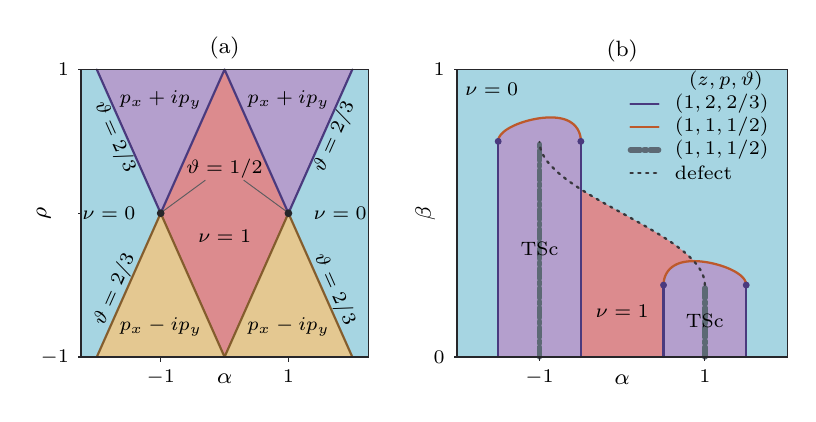
\begin{tikzpicture}[
  every node/.style={font=\fontsize{7.6}{8.2}\selectfont},
  phase label/.style={font=\fontsize{7.2}{7.8}\selectfont},
  critical label/.style={font=\fontsize{6.9}{7.5}\selectfont},
  tick label/.style={font=\fontsize{6.8}{7.4}\selectfont},
  axis label/.style={font=\fontsize{8.3}{8.9}\selectfont},
  panel label/.style={font=\fontsize{8.4}{9.0}\selectfont},
  phase boundary/.style={line width=0.78pt,line cap=round,line join=round},
  cap boundary/.style={capboundary,solid,line width=0.82pt,
                       line cap=round,line join=round},
  zero bulk/.style={zerolocus,dash pattern=on 3.6pt off 1.3pt on 0.9pt off 1.3pt,
                    line width=2.00pt,line cap=round,line join=round},
  defect locus/.style={defectboundary,dotted,line width=0.82pt,
                       line cap=round,line join=round},
]

% Panel (a): beta=0 in the (alpha,rho) plane.
\begin{scope}[shift={(1.85cm,2.20cm)},x=0.81111cm,y=1.825cm]
  \def\A{2.25}
  \def\R{1}

  \fill[nuzerophase] (-\A,-\R) rectangle (\A,\R);
  \fill[nuonephase] (-1,0)--(0,1)--(1,0)--(0,-1)--cycle;
  \foreach \s in {-1,1}{
    \fill[pplusphase] (\s,0)--({\s-\R},\R)--({\s+\R},\R)--cycle;
    \fill[pminusphase] (\s,0)--({\s-\R},-\R)--({\s+\R},-\R)--cycle;
  }
  \draw[phase boundary,pplusboundary]
    (-1,0)--({-1-\R},\R)
    (-1,0)--(0,1)--(1,0)
    (1,0)--({1+\R},\R);
  \draw[phase boundary,pminusboundary]
    (-1,0)--({-1-\R},-\R)
    (-1,0)--(0,-1)--(1,0)
    (1,0)--({1+\R},-\R);

  \node[phase label] at (-1,0.79) {$p_x+i p_y$};
  \node[phase label] at (1,0.79) {$p_x+i p_y$};
  \node[phase label] at (-1,-0.79) {$p_x-i p_y$};
  \node[phase label] at (1,-0.79) {$p_x-i p_y$};
  \node[phase label] at (0,-0.16) {$\nu=1$};
  \node[phase label] at (-1.81,0) {$\nu=0$};
  \node[phase label] at (1.81,0) {$\nu=0$};

  \node[critical label,rotate=-66] at (-1.72,0.53)
    {$\vartheta=2/3$};
  \node[critical label,rotate=66] at (1.72,0.53)
    {$\vartheta=2/3$};
  \node[critical label,rotate=66] at (-1.72,-0.53)
    {$\vartheta=2/3$};
  \node[critical label,rotate=-66] at (1.72,-0.53)
    {$\vartheta=2/3$};

  \node[critical label] at (0,0.31) {$\vartheta=1/2$};
  \draw[axiscolor!75,line width=0.34pt] (-0.30,0.23)--(-0.96,0.015);
  \draw[axiscolor!75,line width=0.34pt] (0.30,0.23)--(0.96,0.015);
  \fill[axiscolor] (-1,0) circle[radius=1.4pt];
  \fill[axiscolor] (1,0) circle[radius=1.4pt];

  \draw[axiscolor,line width=0.52pt] (-\A,-\R) rectangle (\A,\R);
  \foreach \x in {-1,1}{
    \draw[axiscolor,line width=0.44pt] (\x,-\R)--++(0,-0.032);
    \node[below,tick label] at (\x,-\R-0.025) {$\x$};
  }
  \foreach \y/\lab in {-1/$-1$,0/$ $,1/$1$}{
    \draw[axiscolor,line width=0.44pt] (-\A,\y)--++(-0.040,0);
    \node[left,tick label] at (-\A-0.035,\y) {\lab};
  }
  \node[below,axis label] at (0,-\R-0.05) {$\alpha$};
  \node[rotate=90,axis label] at (-\A-0.58,0) {$\rho$};
  \node[panel label] at (0,\R+0.15) {(a)};
\end{scope}

% Panel (b): beta deformation at rho=1/2.
\begin{scope}[shift={(6.90cm,0.375cm)},x=1.05cm,y=3.65cm]
  \def\B{2}
  \fill[nuzerophase] (-\B,0) rectangle (\B,1);

  % Gapped texture sector continuously connected to nu=1 at beta=0.
  \path[fill=nuonephase]
    (-0.5,0)--(0.5,0)--(0.5,0.25)
    -- plot[domain=0.25:0.333333,samples=100,smooth,variable=\t]
       ({sin(360*\t)-sqrt(max(0,0.25-pow(cos(360*\t),2)))},{\t})
    -- plot[domain=0.333333:0.583333,samples=140,smooth,variable=\t]
       ({sin(360*\t)},{\t})
    --(-0.5,0.583333)--cycle;

  \path[fill=pplusphase]
    (0.5,0)--(1.5,0)--(1.5,0.25)
    -- plot[domain=0.25:0.333333,samples=100,smooth,variable=\t]
       ({sin(360*\t)+sqrt(max(0,0.25-pow(cos(360*\t),2)))},{\t})
    -- plot[domain=0.333333:0.25,samples=100,smooth,variable=\t]
       ({sin(360*\t)-sqrt(max(0,0.25-pow(cos(360*\t),2)))},{\t})
    --cycle;
  \path[fill=pplusphase]
    (-1.5,0)--(-0.5,0)--(-0.5,0.75)
    -- plot[domain=0.75:0.833333,samples=100,smooth,variable=\t]
       ({sin(360*\t)+sqrt(max(0,0.25-pow(cos(360*\t),2)))},{\t})
    -- plot[domain=0.833333:0.75,samples=100,smooth,variable=\t]
       ({sin(360*\t)-sqrt(max(0,0.25-pow(cos(360*\t),2)))},{\t})
    --cycle;

  \foreach \x in {0.5,1.5}{
    \draw[phase boundary,pplusboundary] (\x,0)--(\x,0.25);
  }
  \foreach \x in {-1.5,-0.5}{
    \draw[phase boundary,pplusboundary] (\x,0)--(\x,0.75);
  }
  \draw[cap boundary]
    plot[domain=0.25:0.333333,samples=100,smooth,variable=\t]
      ({sin(360*\t)-sqrt(max(0,0.25-pow(cos(360*\t),2)))},{\t})
    -- plot[domain=0.333333:0.25,samples=100,smooth,variable=\t]
      ({sin(360*\t)+sqrt(max(0,0.25-pow(cos(360*\t),2)))},{\t});
  % Zero-rho trap-critical and defect skeleton.  For rho=1/2, the exposed
  % defect segment is the subset 1/3 <= beta <= 7/12 of this same locus.
  \draw[zero bulk] (1,0)--(1,0.25);
  \draw[zero bulk] (-1,0)--(-1,0.75);
  \draw[defect locus]
    plot[domain=0.25:0.75,samples=220,smooth,variable=\t]
      ({sin(360*\t)},{\t});
  \draw[cap boundary]
    plot[domain=0.75:0.833333,samples=100,smooth,variable=\t]
      ({sin(360*\t)-sqrt(max(0,0.25-pow(cos(360*\t),2)))},{\t})
    -- plot[domain=0.833333:0.75,samples=100,smooth,variable=\t]
      ({sin(360*\t)+sqrt(max(0,0.25-pow(cos(360*\t),2)))},{\t});
  \foreach \x/\y in {0.5/0.25,1.5/0.25,-1.5/0.75,-0.5/0.75}{
    \fill[pplusboundary] (\x,\y) circle[radius=1.25pt];
  }

  \node[phase label] at (1.00,0.125) {$\mathrm{TSc}$};
  \node[phase label] at (-1.00,0.375) {$\mathrm{TSc}$};
  \node[phase label] at (0.00,0.16) {$\nu=1$};
  \node[phase label] at (-1.58,0.93) {$\nu=0$};

  % Compact key for the two trap-scaling boundaries and the defect locus.
  \node[critical label,anchor=east] at (1.82,0.96) {$(z,p,\vartheta)$};
  \draw[phase boundary,pplusboundary] (0.10,0.88)--(0.44,0.88);
  \node[critical label,anchor=west] at (0.52,0.88) {$(1,2,2/3)$};
  \draw[cap boundary] (0.10,0.80)--(0.44,0.80);
  \node[critical label,anchor=west] at (0.52,0.80) {$(1,1,1/2)$};
  \draw[zero bulk] (0.10,0.72)--(0.44,0.72);
  \node[critical label,anchor=west] at (0.52,0.72) {$(1,1,1/2)$};
  \draw[defect locus] (0.10,0.64)--(0.44,0.64);
  \node[critical label,anchor=west] at (0.52,0.64) {defect};

  \draw[axiscolor,line width=0.52pt] (-\B,0) rectangle (\B,1);
  \foreach \x in {-1,1}{
    \draw[axiscolor,line width=0.44pt] (\x,0)--++(0,-0.0135);
    \node[below,tick label] at (\x,-0.011) {$\x$};
  }
  \foreach \y/\lab in {0/$0$,1/$1$}{
    \draw[axiscolor,line width=0.44pt] (-\B,\y)--++(-0.036,0);
    \node[left,tick label] at (-\B-0.030,\y) {\lab};
  }
  \node[below,axis label] at (0,-0.03) {$\alpha$};
  \node[rotate=90,axis label] at (-\B-0.38,0.5) {$\beta$};
  \node[panel label] at (0,1.065) {(b)};
\end{scope}

\end{tikzpicture}
\end{document}
